\documentclass[UTF8,a4paper,10pt]{ctexart}
\usepackage[margin=19mm,top=20mm,bottom=20mm]{geometry}
\usepackage{amsmath,amssymb,booktabs,tabularx,graphicx,xcolor,fancyhdr,enumitem}
\usepackage[colorlinks=true,urlcolor=teal,linkcolor=teal]{hyperref}
\definecolor{ink}{HTML}{142B43}\definecolor{accent}{HTML}{168579}\definecolor{teal}{HTML}{168579}
\pagestyle{fancy}\fancyhf{}\fancyhead[L]{\small CF2026 Project 2 · CogAlpha 独立研究}\fancyhead[R]{\small 青序量化平台}
\fancyfoot[L]{\scriptsize 机制复现 / 同预算消融 / 独立去冗余改进}\fancyfoot[R]{\thepage}
\setlength{\headheight}{15pt}\setlength{\parskip}{5pt}\setlength{\parindent}{2em}\setlength{\emergencystretch}{2em}
\setlist{nosep,leftmargin=1.7em}\ctexset{section={format=\Large\bfseries\color{ink}},subsection={format=\normalsize\bfseries\color{accent}}}
\newcommand{\lead}[1]{\par\noindent{\bfseries\color{accent}#1}\par}
\newcommand{\page}[1]{\newpage\section*{#1}}
\begin{document}
\begin{center}{\small\color{accent}COMPUTATIONAL FINANCE / PROJECT 2}\\[9pt]
{\Huge\bfseries\color{ink}CogAlpha 因子研发研究}\\[7pt]
{\Large 受限机制复现、同预算进化对照与去冗余改进}\\[8pt]
2026年10月19日\quad 截止：2026年11月1日
\end{center}


12412408 胡博文；12410819 谢明飞；12410436 王天希\par

\section*{1\quad 摘要与研究结论}

本项目独立研究 Cognitive Alpha Mining via LLM-Driven Code-Based Evolution。我们把七层21角色、因子质量检查、五指标资格判定和变异/交叉机制接入青序平台，采用真实模型提案和已有Tushare快照进行有限规模实验。RSRS路线继续保留；两条研究共享数据、指标、回测和审计基础设施。

\lead{主问题：同样的候选槽位，进化是否优于持续提出新想法？}

三次重复中0/3次测试RankIC提高，平均变化-0.0068，范围-0.0109至-0.0025。

主比较预先固定为LightGBM、测试期平均RankIC、进化49槽相对新提案49槽。两个分支共享21个初代候选，各新增28槽，失败不补位。三个重复全部保留，未按测试成绩选择种子、模型或新参数。

\begin{center}\small\begin{tabularx}{\textwidth}{Xrrr}\toprule
重复 & 新提案RankIC & 进化RankIC & 差值\\\midrule
731 & 0.0656 & 0.0630 & -0.0025\\
732 & 0.0603 & 0.0494 & -0.0109\\
733 & 0.0430 & 0.0361 & -0.0070\\
\bottomrule\end{tabularx}\end{center}

\lead{独立改进：只用训练期IC路径剔除冗余}

三次重复中2/3次测试RankIC提高，平均变化+0.0010，范围-0.0031至+0.0030。

\lead{结论边界}

本实验是不同数据与不同模型规模下的机制复现，不是原文120B模型、H100训练或Table 1/5数值的精确重现。股票池是静态快照；历史已经被研究者看过，模型知识也可能覆盖后续时期。代码层面的未来信息隔离不能把这段历史变成独立盲测。

\page{2\quad 原论文与本次系统：相邻看共同点和差异}

\begin{center}\begin{minipage}[t]{.49\textwidth}\centering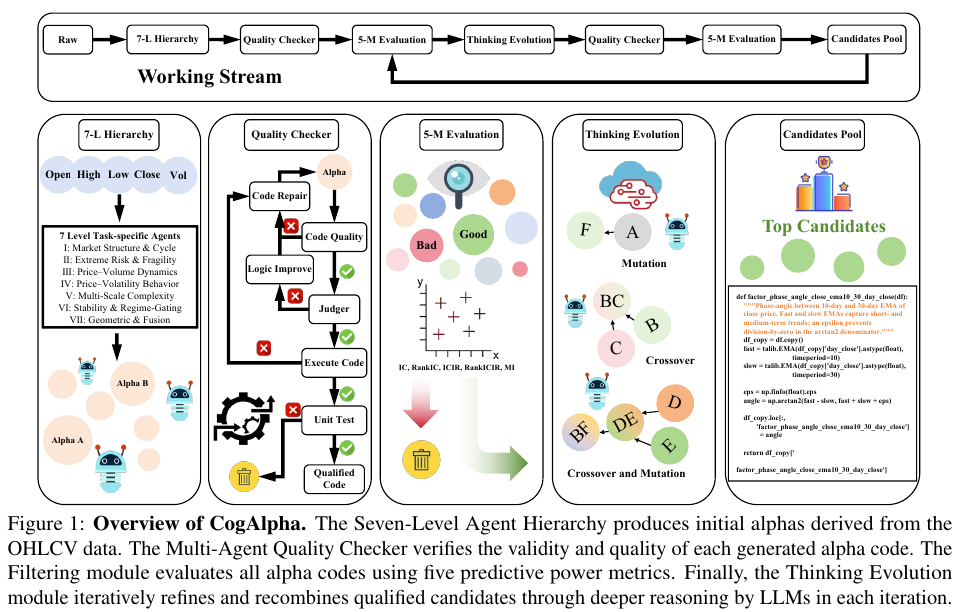
\includegraphics[width=\linewidth,height=77mm,keepaspectratio]{figures/source_figure1.png}\end{minipage}\hfill\begin{minipage}[t]{.49\textwidth}\centering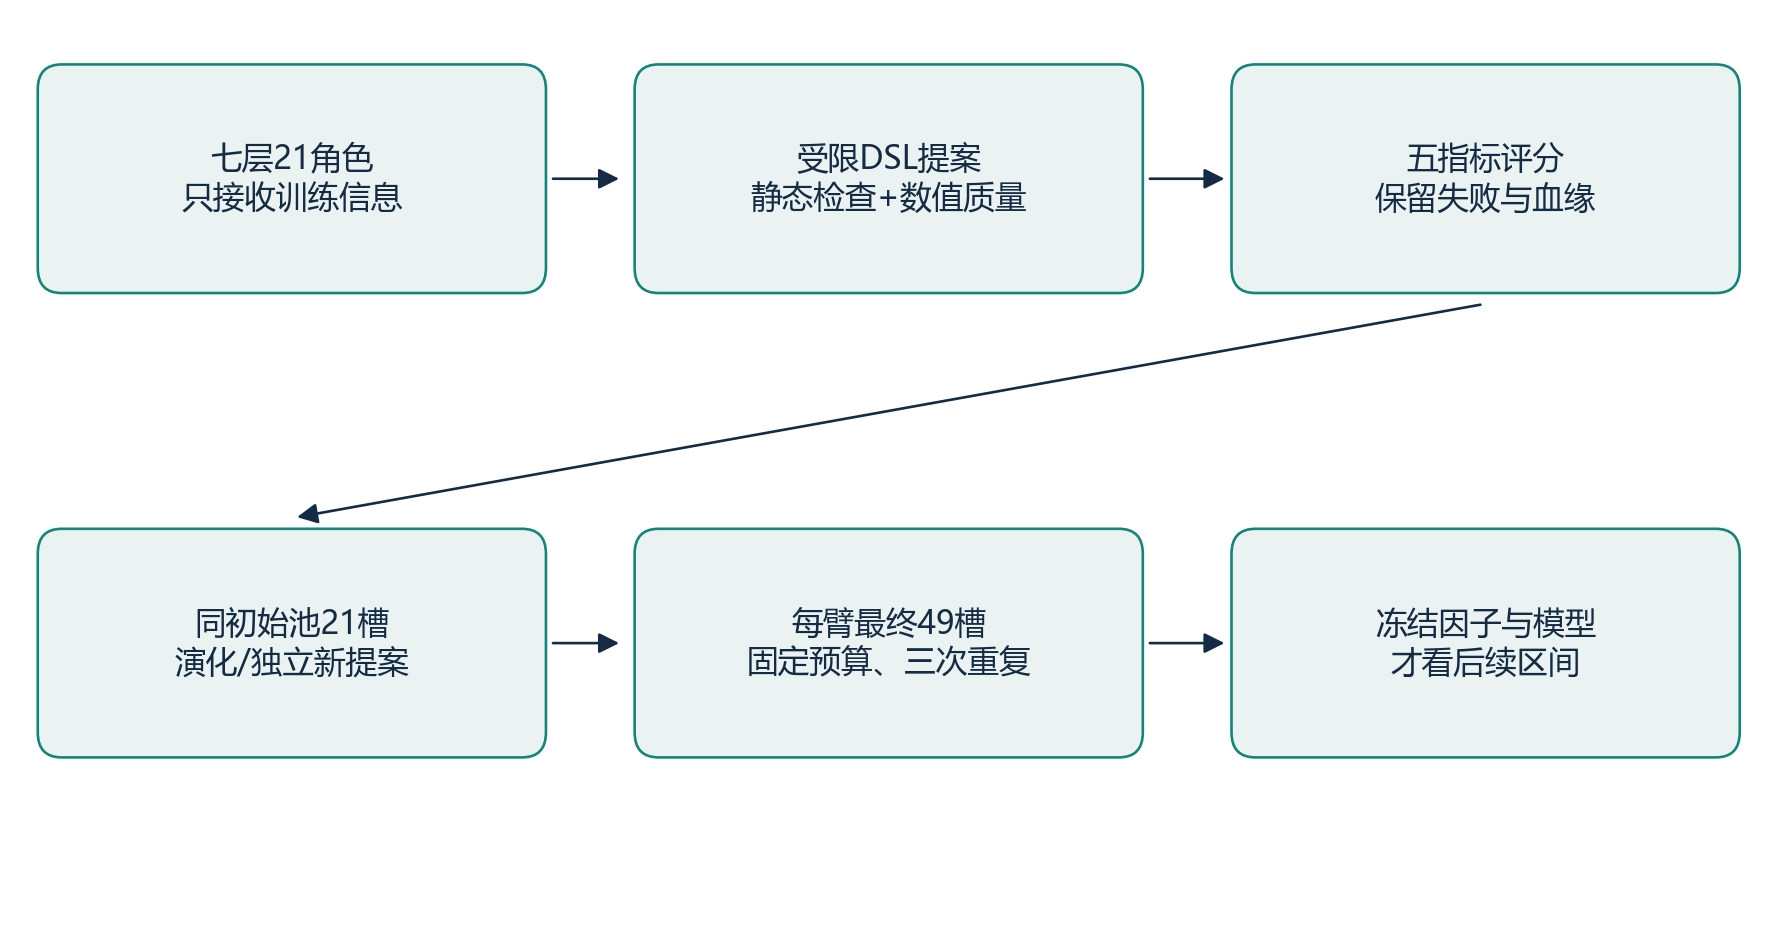
\includegraphics[width=\linewidth,height=77mm,keepaspectratio]{figures/local_workflow.png}\end{minipage}\end{center}

{\footnotesize 左：原文PDF第5页Figure 1；右：青序本次有限工作流。原图为署名文献摘录。}\par

\begin{center}\small\begin{tabularx}{\textwidth}{p{24mm}XX}\toprule
维度 & 原论文 & 本次实验\\\midrule
语言模型 & 本地gpt-oss-120b/H100 & deepseek-flash官方API\\
因子表示 & 生成Python/TA-Lib代码 & 受限OHLCV表达式；不执行任意代码\\
搜索规模 & 初代80、父池32、子池96；多轮 & 21初代+2代；两臂各49槽，三个重复\\
训练方式 & 126日滚动训练 & 训练期拟合一次；后续不重训\\
数据 & Qlib CSI300等多市场 & Tushare静态1000股A股快照\\
公开代码 & 提示词仓库；完整运行时未公开 & 协议、提案血缘、公式、测试与公开汇总\\
\bottomrule\end{tabularx}\end{center}

作者公开仓库仅提供提示词模板，未公开完整运行时、最终20个表达式、数据版本或全部随机状态。本次提示词依据七层角色组织，但数值质量检查、预算账本和安全DSL是青序的工程实现。经济解释是待检验的假设，不是已经观测到的订单流或投资者行为。

\page{3\quad 数据、标签时点与时间隔离}

\begin{center}
\includegraphics[width=.97\textwidth,height=63mm,keepaspectratio]{figures/split_timeline.png}\end{center}

\begin{center}\small\begin{tabularx}{\textwidth}{p{43mm}X}\toprule
字段 & 实际记录\\\midrule
数据日期 & 2019-10-08 00:00:00 至 2026-09-18 00:00:00\\
资产/记录/交易日 & 1000 / 1,656,599 / 1690\\
可用训练日期 & 717\\
最后训练标签退出日 & 2022-12-30 00:00:00\\
\bottomrule\end{tabularx}\end{center}

\[ y_{i,t}^{(10)}=\frac{O^{adj}_{i,t+11}}{O^{adj}_{i,t+1}}-1,\qquad t\text{日收盘形成信号。}\]

训练样本不仅要求形成日在训练区间内，还要求标签退出日严格早于下一切分边界。验证/测试评价同样剔除尚未实现的退出标签；终点附近不凭空补未来收益。因子提案、修复、亲本选择、去冗余和模型拟合都只接收训练统计。

价格按当时复权因子相对首个观测基准调整，成交量按相反比例调整，以保持价格乘成交量的金额口径。缺失OHLCV不向前填充；资格掩码不使用未来标签。1000股静态成员不是历史沪深300成分，因此有幸存者与静态选样偏差。

\page{4\quad 论文示例公式与手算：先确认程序算对了}

\begin{center}\begin{minipage}[t]{.49\textwidth}\centering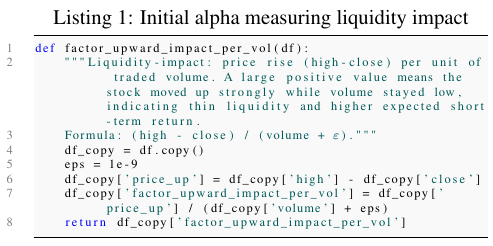
\includegraphics[width=\linewidth,height=67mm,keepaspectratio]{figures/source_listing1.png}\end{minipage}\hfill\begin{minipage}[t]{.49\textwidth}\centering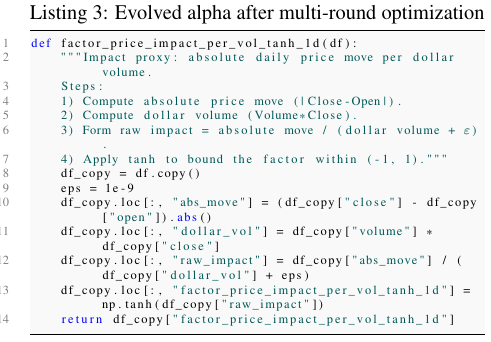
\includegraphics[width=\linewidth,height=67mm,keepaspectratio]{figures/source_listing3.png}\end{minipage}\end{center}

{\footnotesize 左：原文第8页Listing 1；右：第17页Listing 3。第17页Listing 2将第一式的分子改为$H-L$。}\par

\[ f_1=\frac{H-C}{V+\varepsilon},\qquad f_2=\frac{H-L}{V+\varepsilon},\qquad f_3=\tanh\!\left(\frac{|C-O|}{VC+\varepsilon}\right).\]

以教学数值O=10、H=12、L=9、C=11、V=100000股代入；这些数值不是行情样本，也不用于实证。

\begin{center}\small\begin{tabularx}{\textwidth}{Xrrr}\toprule
公式 & 手算值 & DSL执行值 & 检查\\\midrule
Listing 1 & 1e-05 & 1e-05 & 通过\\
Listing 2 & 3e-05 & 3e-05 & 通过\\
Listing 3 & 9.090909091e-07 & 9.090909091e-07 & 通过\\
\bottomrule\end{tabularx}\end{center}

原文epsilon=1e-9；本次实现epsilon=1e-09。数值稳定项一致。

第一式的H-C是最高价至收盘的距离，不等于开盘到收盘的上涨；报告保留源公式，同时指出原经济叙述的歧义。三个示例按正向定义评价，不根据后验表现反转符号。

\page{5\quad 五项评价、资格门槛与受限解释}

\[ IC_t=\operatorname{corr}_i(f_{i,t},y_{i,t}),\quad RankIC_t=\operatorname{corr}_i(\operatorname{rank}f_{i,t},\operatorname{rank}y_{i,t}).\]

\[ ICIR=\overline{IC}/s(IC),\qquad RankICIR=\overline{RankIC}/s(RankIC),\quad ddof=1.\]

预测信息比率不年化。每日横截面至少30个有效配对；均值按有效日期计算。MI采用每日秩五分位离散化的插件估计，以自然对数计量。原文给出互信息定义，但没有公开估计器，故MI是本次明确标注的替代实现，有限样本下可能向上偏。

\begin{center}\small\begin{tabularx}{\textwidth}{lrrrr}\toprule
阶段 & 分位数 & IC / RankIC底线 & ICIR / RankICIR底线 & MI底线\\\midrule
qualified & 65\% & 0.005 & 0.05 & 0.02\\
elite & 80\% & 0.010 & 0.10 & 0.02\\
\bottomrule\end{tabularx}\end{center}

每项实际门槛取池内分位数与绝对底线的较大者，五项全部满足才具资格；本地实现采用大于等于比较，不取绝对值。缺失或非有限值不能通过资格。本次在截至当前槽已评分的累计池上重算分位数，原文描述的是同代候选池；小规模累计池是明确的工程改造，不冒充作者的代际筛选实现。

\lead{资格、工程亲本池和最终建模池分别报告}

进化优先使用qualified且训练RankIC为正的候选，并优先elite。若五项交集为空，允许使用质量通过、训练RankIC为正的工程回退亲本池；每次回退明确标记，绝不改称qualified。最终组合另按预先固定的正训练RankIC顺序选择最多20个因子；论文最终选择细节未公开，因此这也是本地规则。

\lead{安全与时序质量检查}

表达式先通过AST白名单，再检查数值、覆盖率和因果性。最大单窗口120日；禁止任意代码、属性访问和未来位移。前缀重算与未来扰动检查都在训练窗口完成，覆盖率至少70\%。通过这些检查说明计算边界满足要求，不等于因子有经济价值。

\page{6\quad 同预算对照、失败槽与真实调用}

\begin{center}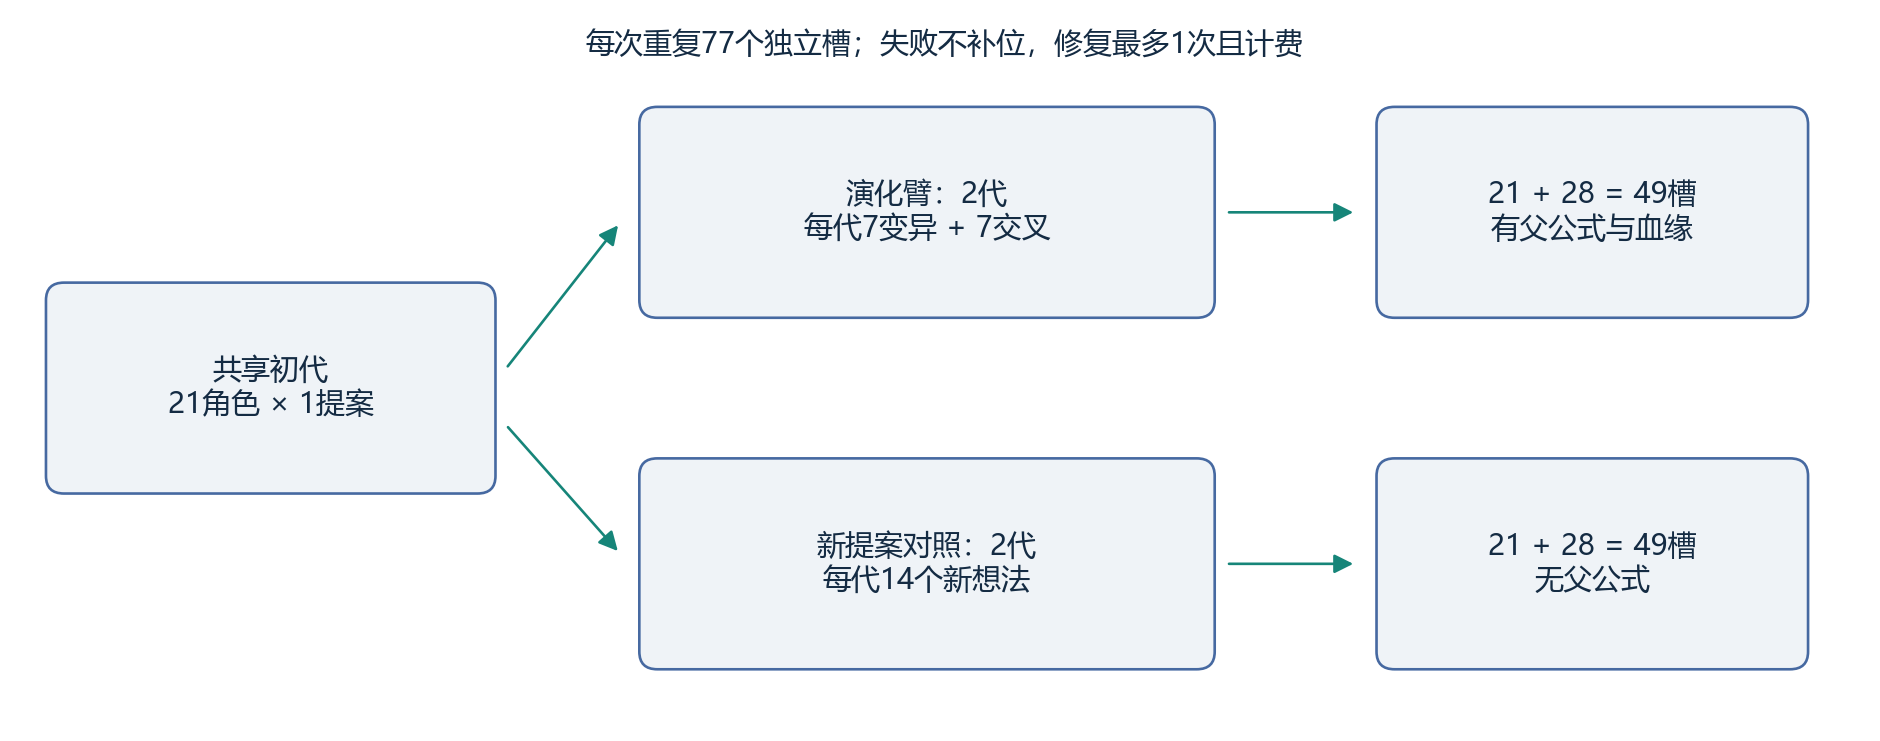
\includegraphics[width=.97\textwidth,height=66mm,keepaspectratio]{figures/matched_budget.png}\end{center}

\begin{center}\small\begin{tabularx}{\textwidth}{lrrrrrr}\toprule
重复 & 独立槽 & 通过 & 拒绝 & 请求尝试 & 修复槽 & 回退亲本\\\midrule
731 & 77 & 60 & 17 & 78 & 1 & 0\\
732 & 77 & 66 & 11 & 78 & 1 & 0\\
733 & 77 & 71 & 6 & 80 & 3 & 28\\
\bottomrule\end{tabularx}\end{center}

同预算指相同的候选槽位上限：两臂都从共享21槽扩展到49槽。新提案对照获得同类训练统计，不获得父公式。重复表达式、无效公式和API失败均占用原槽且保留；每槽最多一次修复且计费，因此实际调用数及费用可能不同，不能声称token完全相同。

\begin{center}\small\begin{tabularx}{\textwidth}{p{60mm}X}\toprule
预算项 & 实际账本\\\midrule
全局费用上限 & 50.00元\\
全局调用/成功 & 237 / 237\\
成功请求计费 & 1.312712元\\
不确定请求保守预留 & 0.000000元\\
总已花或预留 & 1.312712元\\
\bottomrule\end{tabularx}\end{center}

预算为三个重复、连接检查及修复共同使用；失败请求按保守上界保留预算，预留不等于已确认账单。每次请求保存namespace、请求哈希和响应模型字段。父因子抽样使用本地种子，但API模型采样没有可控seed；缓存提供请求级复现，不能保证重新付费生成相同表达式。

请求别名是deepseek-flash；官网2026年10月19日映射为DeepSeek-V4.1-Flash-1017。响应中的model字段只证明返回的名称，不独立证明不可变checkpoint；无法钉死服务端权重。原始响应与冻结公式保留后可离线重评。

{\footnotesize 模型身份来源：\url{https://api-docs.deepseek.com/quick_start/pricing}，当日首次调用页模型表脚注。}\par

\page{7\quad 候选池与最终选择：保留全部重复}

\begin{center}\scriptsize\begin{tabularx}{\textwidth}{lp{29mm}rrrrrr}\toprule
重复 & 候选臂 & 槽位 & 质量通过 & qualified & elite & 正RankIC & 入模\\\midrule
0 & 固定16因子 & 16 & 16 & 1 & 0 & 6 & 6\\
0 & Listing 1 & 1 & 1 & 0 & 0 & 1 & 1\\
0 & Listing 2 & 1 & 1 & 0 & 0 & 1 & 1\\
0 & Listing 3 & 1 & 1 & 1 & 0 & 1 & 1\\
731 & 初代21槽 & 21 & 21 & 1 & 0 & 8 & 8\\
731 & 独立新提案49槽 & 49 & 48 & 2 & 0 & 20 & 20\\
731 & 进化49槽 & 49 & 33 & 6 & 0 & 20 & 20\\
731 & 进化+去冗余 & 49 & 33 & 6 & 0 & 20 & 9\\
732 & 初代21槽 & 21 & 21 & 1 & 1 & 7 & 7\\
732 & 独立新提案49槽 & 49 & 49 & 2 & 0 & 20 & 20\\
732 & 进化49槽 & 49 & 38 & 8 & 0 & 24 & 20\\
732 & 进化+去冗余 & 49 & 38 & 8 & 0 & 24 & 8\\
733 & 初代21槽 & 21 & 20 & 0 & 0 & 11 & 11\\
733 & 独立新提案49槽 & 49 & 47 & 0 & 0 & 20 & 20\\
733 & 进化49槽 & 49 & 44 & 0 & 0 & 29 & 20\\
733 & 进化+去冗余 & 49 & 44 & 0 & 0 & 29 & 14\\
\bottomrule\end{tabularx}\end{center}

“正RankIC”指训练期平均RankIC大于零的质量通过候选数。质量通过只说明公式可计算且符合时序检查；qualified/elite要求五项共同达标；最终入模另按正训练RankIC排序、最多20个，去冗余臂再过滤相关路径。三种选择层级不能混称。论文三个字面公式作为独立基准原向执行，不因训练符号而删去。不可得值、拒绝理由、代数和父ID均在公开血缘记录中保留。

\lead{同预算对照解释的边界}

两个分支共享初代，重复检测在各臂内部执行，防止一条分支先提出某公式就额外惩罚另一条分支。相同槽位不消除随机模型输出差异；三个重复用于检查方向和离散程度，不足以声称统计显著或全市场稳定。

\page{8\quad 固定组合模型与组合交易}

\begin{center}\small\begin{tabularx}{\textwidth}{p{30mm}X}\toprule
项目 & 本次固定口径\\\midrule
因子/标签缩放 & 同日合资格横截面秩减0.5\\
rank组合 & 选定因子的等权平均秩\\
Ridge & alpha=100\\
LightGBM & 200树，15叶，深度5，学习率0.05\\
拟合/选择 & 只用训练期；不在验证期再训练或改变选择\\
持仓与调仓 & Top50/Drop5，保留继续持有股票的原份额\\
成交与费用 & 收盘t评分，t+1开盘成交；买0.05\%、卖0.15\%，单笔最低5元\\
账户/年化 & 初始100万元，现金收益0；252交易日，无风险年利率0\\
\bottomrule\end{tabularx}\end{center}

论文也采用Top50/Drop5、开盘交易与上述费用；本次复用青序成交和现金账本，使用分数化复权研究份额，不等同A股整手订单。继续持有的股票不每天重置为等权，以免人为增加换手。

撮合按下一开盘价执行，缺失开盘或涨跌停价则阻止该笔交易；依据Tushare涨跌停价，开盘触及涨停禁止买、触及跌停禁止卖。未成交卖单仍占持仓槽。缺失收盘使用此前收盘估值，连续缺失超过20个交易日按零记账，这是研究中的保守减记规则，不是实际清算结果。未启用成交参与率限制，也未模拟整手、订单排队、冲击或额外滑点。资格池另用涨跌停比率排除类似5\%限制的股票，只是ST-like代理，并非完整历史ST识别。

\[ Sharpe=\sqrt{252}\,\frac{\overline{r^{net}}}{s(r^{net})},\qquad AER=252\,\overline{(r^{net}-r^{bench})}.\]

CAGR采用复利年化；AER是平均日超额收益的算术年化，两者不能混用。最大回撤包含初始资金峰值。沪深300是免交易费的价格指数代理，从同一评价首日开盘归一化；它不是可直接购买的ETF或含分红全收益基准。股票侧采用复权总收益研究单位，因此相对该价格指数的AER不等于相对沪深300全收益指数的alpha，分红口径可能贡献差异。

验证区间的预测从首个验证交易日收盘开始，因此第一天账户持有现金、最早下一开盘交易；测试区间已有前期预测信号。没有为了补齐首日交易而使用当日收盘分数在当日开盘成交。

\page{9\quad 主实验：进化49槽对独立新提案49槽}

\begin{center}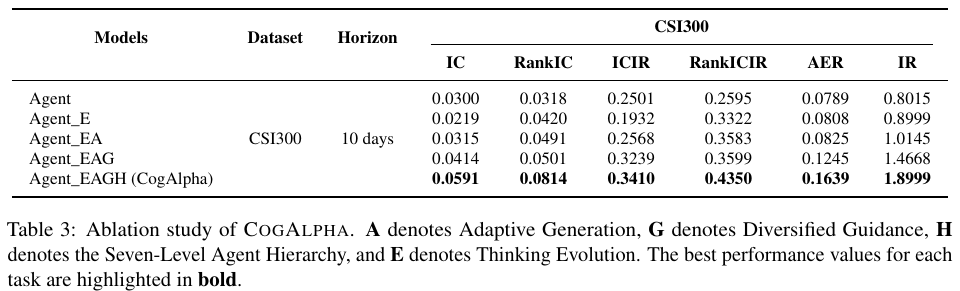
\includegraphics[width=.97\textwidth,height=51mm,keepaspectratio]{figures/source_table3.png}\end{center}

{\footnotesize 原文第16页Table 3：Agent到Agent\_E的RankIC由0.0318升到0.0420，但IC由0.0300降到0.0219。原表不是本次同槽位对照。}\par

\begin{center}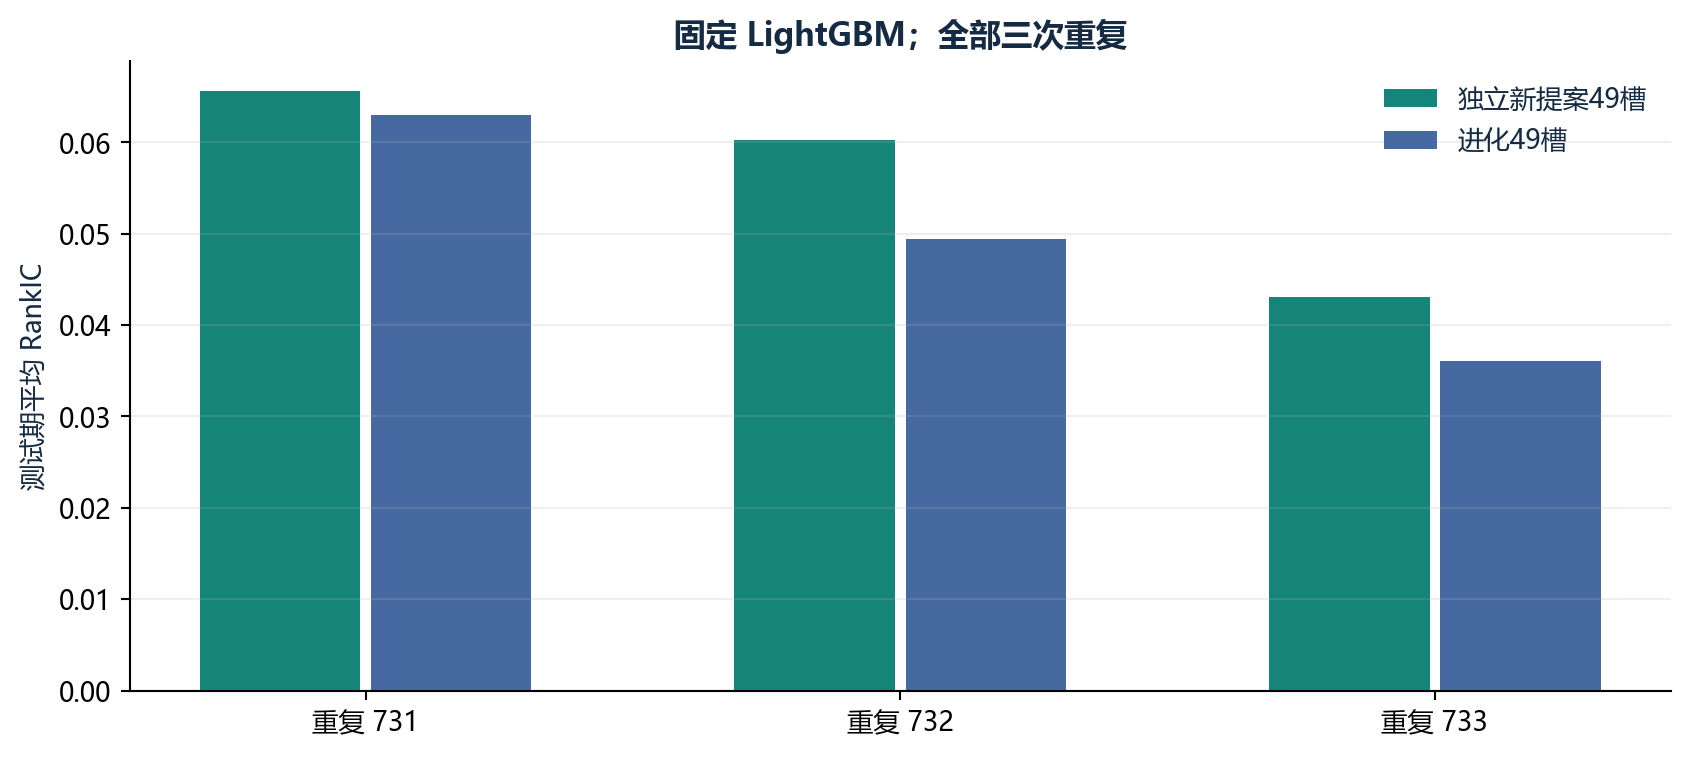
\includegraphics[width=.97\textwidth,height=72mm,keepaspectratio]{figures/primary_rankic.png}\end{center}

三次重复中0/3次测试RankIC提高，平均变化-0.0068，范围-0.0109至-0.0025。

\begin{center}\small\begin{tabularx}{\textwidth}{lrrrrr}\toprule
重复 & 新提案RankIC & 进化RankIC & 差值 & CAGR变化(pp) & Sharpe变化\\\midrule
731 & 0.0656 & 0.0630 & -0.0025 & +1.99 & +0.140\\
732 & 0.0603 & 0.0494 & -0.0109 & -9.61 & -0.328\\
733 & 0.0430 & 0.0361 & -0.0070 & +5.29 & +0.344\\
\bottomrule\end{tabularx}\end{center}

这里的差值都取进化减新提案，保持数据、模型、交易规则和最终选择上限一致。RankIC检验横截面排序能力，CAGR与Sharpe检验交易后的账户表现；二者方向可能不同。收益下降的重复不能被删去，也不能改用表现最好的模型来替换主比较。

本次两臂都保留七层组织及训练统计反馈，检验的差别是是否提供父公式并做变异/交叉，并未分别识别原文全部模块。三个种子不是三个独立市场样本，不凭这三个观察点作显著性或未来盈利保证。

\page{10\quad 原表与本次结果相邻：只作有条件的比较}

\begin{center}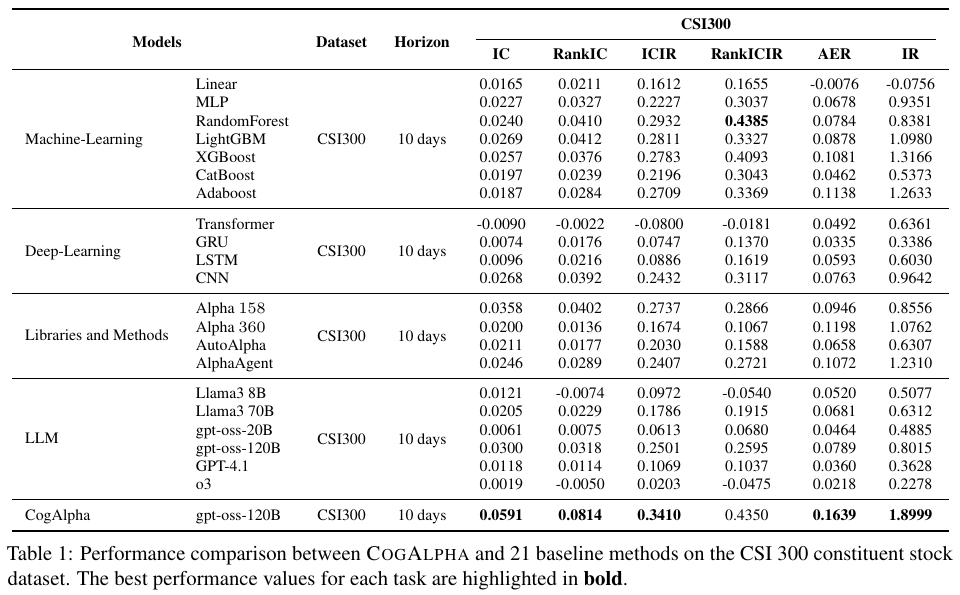
\includegraphics[width=.97\textwidth,height=104mm,keepaspectratio]{figures/source_table1.png}\end{center}

{\footnotesize 原文PDF第7页Table 1完整摘录；CSI300，10日标签，原论文训练/测试区间。}\par

\begin{center}\small\begin{tabularx}{\textwidth}{Xrrrr}\toprule
来源/配置 & IC & RankIC & ICIR & RankICIR\\\midrule
原文CogAlpha & 0.0591 & 0.0814 & 0.3410 & 0.4350\\
本次进化/731 & 0.0208 & 0.0630 & 0.1266 & 0.3724\\
本次进化/732 & 0.0183 & 0.0494 & 0.1184 & 0.3105\\
本次进化/733 & 0.0086 & 0.0361 & 0.0708 & 0.3217\\
\bottomrule\end{tabularx}\end{center}

两组使用不同股票池、日期、模型、训练频率、搜索规模和指标估计细节，因此不计算直接复现误差或对原文提升百分比。本次可识别的比较是同一冻结数据内的进化与新提案对照；原表提供研究定位，不能作为可达到收益的承诺。

\page{11\quad 扣费净值：全部三个重复同样展示}

\begin{center}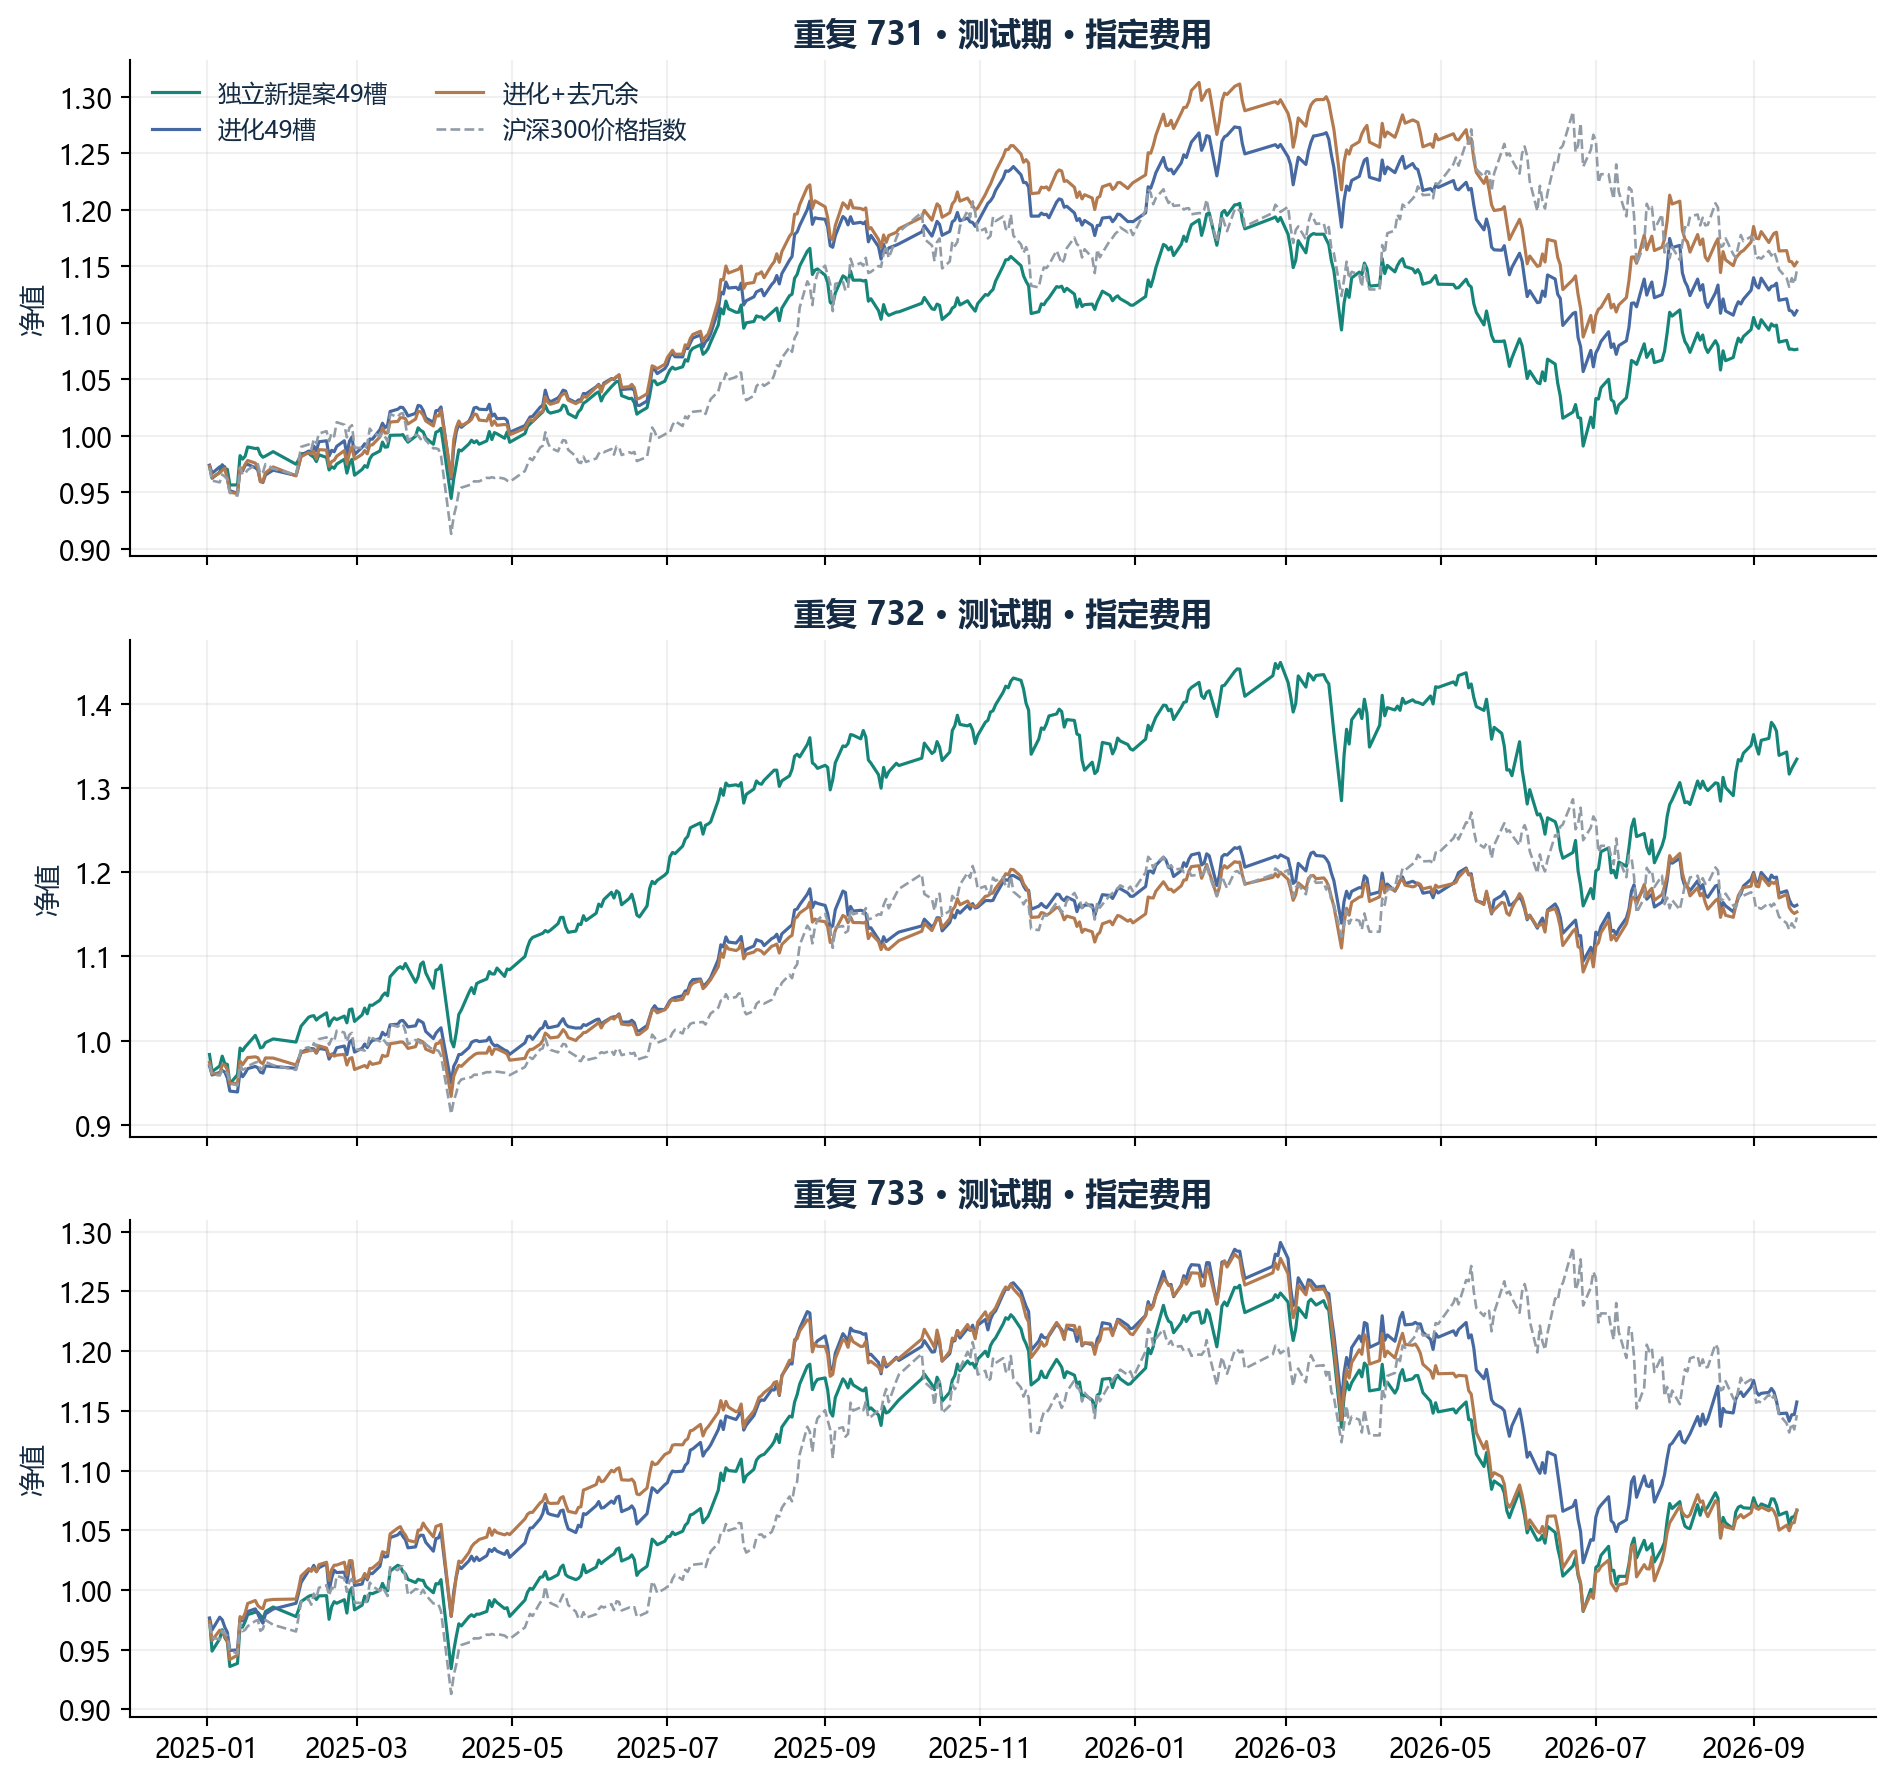
\includegraphics[width=.97\textwidth,height=194mm,keepaspectratio]{figures/portfolio_all_seeds.png}\end{center}

所有曲线使用测试期和指定费用；各自账户均从初始资金开始。股票侧是复权总收益研究单位，沪深300侧是免交易费价格指数；两者分红口径不同。这里跑赢价格指数不能等同于跑赢沪深300全收益基准。净值好坏不改变此前冻结的因子或模型选择；主比较RankIC不依赖该指数基准。

\page{12\quad 独立改进：训练期IC路径去冗余}

\begin{center}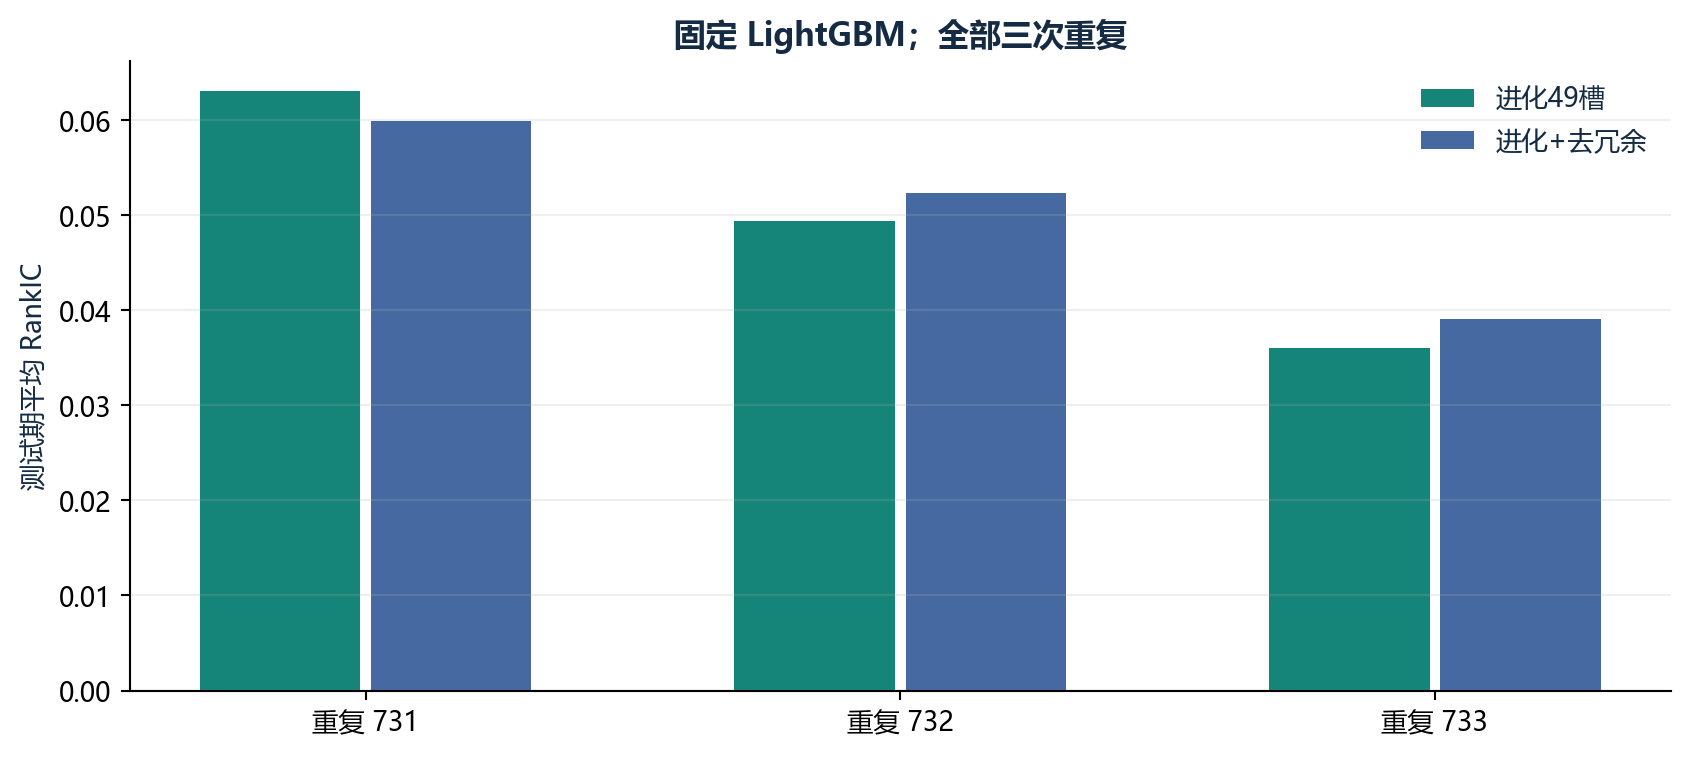
\includegraphics[width=.97\textwidth,height=80mm,keepaspectratio]{figures/diverse_rankic.png}\end{center}

在进化候选池不变的条件下，按正训练RankIC排序逐一加入因子；若与已选因子训练期每日RankIC序列的绝对相关超过0.8，则跳过。最多20个；相关不可得或有效共同日期不足也跳过。此规则与市场条件、测试收益无关，未在测试上寻找最优阈值。

\begin{center}\small\begin{tabularx}{\textwidth}{lrrrrr}\toprule
重复 & 原进化RankIC & 去冗余RankIC & RankIC变化 & CAGR变化(pp) & 回撤变化(pp)\\\midrule
731 & 0.0630 & 0.0600 & -0.0031 & +2.47 & +0.16\\
732 & 0.0494 & 0.0524 & +0.0030 & -0.46 & -0.23\\
733 & 0.0361 & 0.0390 & +0.0030 & -5.23 & +2.55\\
\bottomrule\end{tabularx}\end{center}

三次重复中2/3次测试RankIC提高，平均变化+0.0010，范围-0.0031至+0.0030。

回撤变化按新减旧，负值表示回撤幅度降低。训练IC路径不高度相关，并不保证因子值、预测误差或最终持仓完全独立；入模数量也可能同时减少，应连同候选池表解释。我们不把去冗余结果自动提升为平台默认策略。

\page{13\quad 模型与费用敏感性：不替换主比较}

\begin{center}\scriptsize\begin{tabularx}{\textwidth}{llrrrr}\toprule
重复 & 组合模型 & 新提案RankIC & 进化RankIC & 差值 & CAGR变化(pp)\\\midrule
731 & rank & 0.0395 & 0.0335 & -0.0059 & -8.78\\
732 & rank & 0.0403 & 0.0318 & -0.0085 & -15.71\\
733 & rank & 0.0202 & 0.0013 & -0.0189 & +3.80\\
731 & ridge & 0.0471 & 0.0473 & +0.0002 & -6.26\\
732 & ridge & 0.0491 & 0.0353 & -0.0138 & -4.43\\
733 & ridge & 0.0257 & 0.0324 & +0.0067 & -1.88\\
731 & lightgbm & 0.0656 & 0.0630 & -0.0025 & +1.99\\
732 & lightgbm & 0.0603 & 0.0494 & -0.0109 & -9.61\\
733 & lightgbm & 0.0430 & 0.0361 & -0.0070 & +5.29\\
\bottomrule\end{tabularx}\end{center}

rank、Ridge与LightGBM使用同一候选池和训练期规则。上表用于理解组合器的影响；主比较仍为LightGBM，不把其中最好的行改成事后主结论。pp表示百分点，报告中收益率与回撤差值均按百分点表示。

\begin{center}\scriptsize\begin{tabularx}{\textwidth}{lXrrrr}\toprule
重复 & 工程基线/初代 & RankIC & CAGR & Sharpe & 回撤\\\midrule
0 & 固定16因子 & 0.0455 & 3.27\% & 0.292 & 16.27\%\\
731 & 初代21槽 & 0.0608 & 6.59\% & 0.536 & 17.79\%\\
732 & 初代21槽 & 0.0535 & 9.00\% & 0.653 & 12.83\%\\
733 & 初代21槽 & 0.0369 & 3.15\% & 0.283 & 21.14\%\\
\bottomrule\end{tabularx}\end{center}

上表同为LightGBM、测试期与指定费用。固定16因子是本地工程基线，不等同论文的Alpha158；初代行显示增加提案前的结果，不能把与初代的差异全部归因于演化。

\begin{center}\small\begin{tabularx}{\textwidth}{lXrrr}\toprule
重复 & 候选臂 & 零费CAGR & 指定费CAGR & 成本后变化(pp)\\\midrule
731 & 独立新提案49槽 & 9.91\% & 4.55\% & -5.36\\
731 & 进化49槽 & 12.03\% & 6.54\% & -5.49\\
732 & 独立新提案49槽 & 25.35\% & 19.05\% & -6.30\\
732 & 进化49槽 & 14.43\% & 9.44\% & -4.99\\
733 & 独立新提案49槽 & 9.36\% & 3.95\% & -5.41\\
733 & 进化49槽 & 14.98\% & 9.23\% & -5.75\\
\bottomrule\end{tabularx}\end{center}

零费与指定费用是敏感性实验，扣费后路径会因可用现金和持仓演化而改变，不能把两条终值差简单等同于累计手续费。两种费用都不影响预测RankIC，因为预测分数与标签没有变。

\page{14\quad 示例因子与单因子实验}

\begin{center}\small\begin{tabularx}{\textwidth}{Xrrrrr}\toprule
原公式 & 本次测试IC & RankIC & CAGR & Sharpe & 回撤\\\midrule
Listing 1 & 0.0187 & 0.0182 & 10.54\% & 0.580 & 20.81\%\\
Listing 2 & 0.0187 & 0.0153 & 11.80\% & 0.606 & 20.10\%\\
Listing 3 & 0.0216 & 0.0234 & 21.20\% & 1.066 & 19.92\%\\
\bottomrule\end{tabularx}\end{center}

论文报告Listing 1/2/3的示例IC分别为0.0090、0.0073、0.0141，RankIC为0.0061、0.0021、0.0087，但该示例的完整样本和筛选历史未公开。本次只比较同一数据上的原公式形状，不宣称还原作者的这几个数值。单因子未重新训练为多因子模型。

\lead{实际生成表达式：按训练期排序展示，不按测试选例}

\lead{重复731：Downside-realized-volatility share of total range variance}

训练RankIC=0.0317；代数0；操作initial。

{\footnotesize\ttfamily\raggedright safe\_divide(\allowbreak rolling\_std(\allowbreak rolling\_min(\allowbreak close,\allowbreak 5)-delay(\allowbreak close,\allowbreak 5),\allowbreak 20),\allowbreak  rolling\_std(\allowbreak high-low,\allowbreak 20))\par}

Stocks whose recent downside moves dominate their total dispersion may reflect asymmetric selling pressure and loss-aversion-driven repricing; if that pressure is transient, higher values should predict higher next-open-to-10-session returns. The factor compares 20-day…（节选）

\lead{重复732：Composite range-volume compression: low normalized 20d high-low range and low volume dispersion predict higher forward returns}

训练RankIC=0.0346；代数0；操作initial。

{\footnotesize\ttfamily\raggedright -1 * tanh(\allowbreak  rolling\_mean(\allowbreak  safe\_divide(\allowbreak  rolling\_max(\allowbreak high,\allowbreak 20) - rolling\_min(\allowbreak low,\allowbreak 20),\allowbreak  rolling\_mean(\allowbreak close,\allowbreak 20) ),\allowbreak  5 ) + rolling\_std(\allowbreak  safe\_divide(\allowbreak volume,\allowbreak  rolling\_mean(\allowbreak volume,\allowbreak 20)),\allowbreak  20 ) )\par}

Stocks whose recent 20-day price range is narrow relative to their own price level and whose volume is unusually stable (low dispersion of volume relative to its 20-day mean) are in a quiet, low-attention consolidation state. A composite of these two standardized compression…（节选）

\lead{重复733：Rolling range compression then expansion with volume confirmation}

训练RankIC=0.0269；代数0；操作initial。

{\footnotesize\ttfamily\raggedright tanh(\allowbreak rank(\allowbreak safe\_divide(\allowbreak rolling\_std(\allowbreak returns(\allowbreak close,\allowbreak 1),\allowbreak 20),\allowbreak rolling\_mean(\allowbreak abs(\allowbreak returns(\allowbreak close,\allowbreak 1)),\allowbreak 20))) * rank(\allowbreak safe\_divide(\allowbreak volume,\allowbreak rolling\_mean(\allowbreak volume,\allowbreak 20))) * rank(\allowbreak safe\_divide(\allowbreak close,\allowbreak rolling\_max(\allowbreak high,\allowbreak 20))))\par}

When short-horizon realized volatility is compressed relative to its own recent average absolute move, and this compression coincides with elevated volume and price sitting near its 20-day high, the stock is in a coiled state; subsequent expansion in the direction of the…（节选）

\page{15\quad 平台接入、复现路径与验收范围}

青序平台分别展示冻结协议、原文对照、三次重复、候选血缘和账本。因子挖掘作为辅助研究路线保留，未经独立后续验证不自动替换已有策略。阅读已保存的研究结果不需要重新付费调用模型。

\begin{center}\small\begin{tabularx}{\textwidth}{p{28mm}X}\toprule
层次 & 对应实现/证据\\\midrule
数据与因子 & cogalpha.py：指标、质量、原公式和去冗余\\
真实提案 & cogalpha\_mining.py + research\_api.py：槽位、血缘、缓存、共享预算\\
冻结模型 & cogalpha\_models.py：rank/Ridge/LightGBM统一训练边界\\
研究编排 & cogalpha\_study.py；configs/project2\_cogalpha.json\\
P1复用 & 成交、持仓、现金、费用、绩效与账本核对\\
公开证据 & performance/comparison/pool/qualification/lineage/manifest\\
材料 & 报告TeX/PDF、Beamer、可编辑PPTX及逐页讲稿\\
\bottomrule\end{tabularx}\end{center}

\lead{已验证范围}

462项去重自动测试跨已记录环境全部通过；另附独立审计器合成自检

5项界面自动测试通过；最终浏览器操作验收另附记录

正式研究账本核验：90组；all\_ledgers\_passed=True。具体检查逐条见validation.json。

\lead{重跑原则}

先核验协议和输入身份，再复用已有提案缓存执行evaluate阶段。mine/all阶段会在授权的共享预算内产生真实模型调用；阶段区分防止只读验收意外付费。原始Tushare数据、密钥和训练模型不放入公开仓库；公开聚合曲线及哈希支持核对，完整重算仍需要有权限的同版数据。

{\footnotesize\ttfamily python scripts/build\_project2\_cogalpha\_materials.py\par}

\page{16\quad 限制、后续验证和来源}

\lead{不能由当前实验推出的结论}

静态股票池存在幸存者偏差；调整价格和分数化份额不是可成交整手实盘。历史已经看过且LLM可能知道后续市场，时间切分不能完全消除研究者或模型知识污染。只有三次提案重复，不能支撑普遍显著性。MI估计器、最终选择、训练周期、数据和模型均与原文不同。

后续应冻结候选后收集新的时间区间，以历史成分股票池和可交易约束再次验证，并加入分红口径一致的全收益基准、不同市场阶段、手续费与冲击。股票复权单位相对价格指数的超额不能直接解释为全收益基准alpha。若未来表现不佳，保留失败结果；不在同一已见测试期反复调参直到跑赢。

\lead{来源与对应位置}

\begin{enumerate}\item Fengyuan Liu等，\textit{Cognitive Alpha Mining via LLM-Driven Code-Based Evolution}，arXiv:2511.18850v4。Figure 1第5页；Table 1第7页；Listing 1第8页；Figure 2第12页；数据与指标第14--16页；Listing 2/3第17页；Table 5第19页。\url{https://arxiv.org/abs/2511.18850v4}

\item 作者提示词仓库：\url{https://github.com/uwFengyuan/CogAlpha_Prompt}。固定版本见下列身份记录。

\item 本项目冻结配置、输入哈希、公开汇总及完整槽位记录：evidence/project2\_cogalpha。原始图片摘录的页码、裁切范围与哈希见source\_reference.json。\end{enumerate}

\lead{精确身份}

论文文件SHA以独立来源勘误为准；冻结配置保留原字节及运行身份，勘误不改变实验。

{\scriptsize 论文PDF SHA256：\par\ttfamily 20c6c76a0e9ea5fdf869ee0a20a3594ab61181fee9913b1ec9361b3669ecea45\par}

{\scriptsize 提示词仓库commit：\par\ttfamily e6f422ddd8250f03b6c887bcf3a82ce8507c46e4\par}

{\scriptsize 研究身份：\par\ttfamily 5e65b434777e451910a2395c81a9adbd22f5a5db1b44a0a400d54fce61010dc6\par}

本报告保留限制和负面结果，目标是让公式、数据、实验、图表和结论彼此对应。评分由课程教师决定；这些材料不构成未来收益或课程成绩保证。

\end{document}